\subsection{Dyslexia}
Dyslexia is a common learning disability that affects reading and language processing skills. Children with dyslexia often struggle with various aspects of reading, including decoding, spelling, reading comprehension, and phonological memory. Understanding the user profile associated with dyslexia can guide the development of effective mini-games to address the specific goals, psychographics, problems, facts, and needs of children with this learning disability.

\begin{figure}[H]
    \centering
    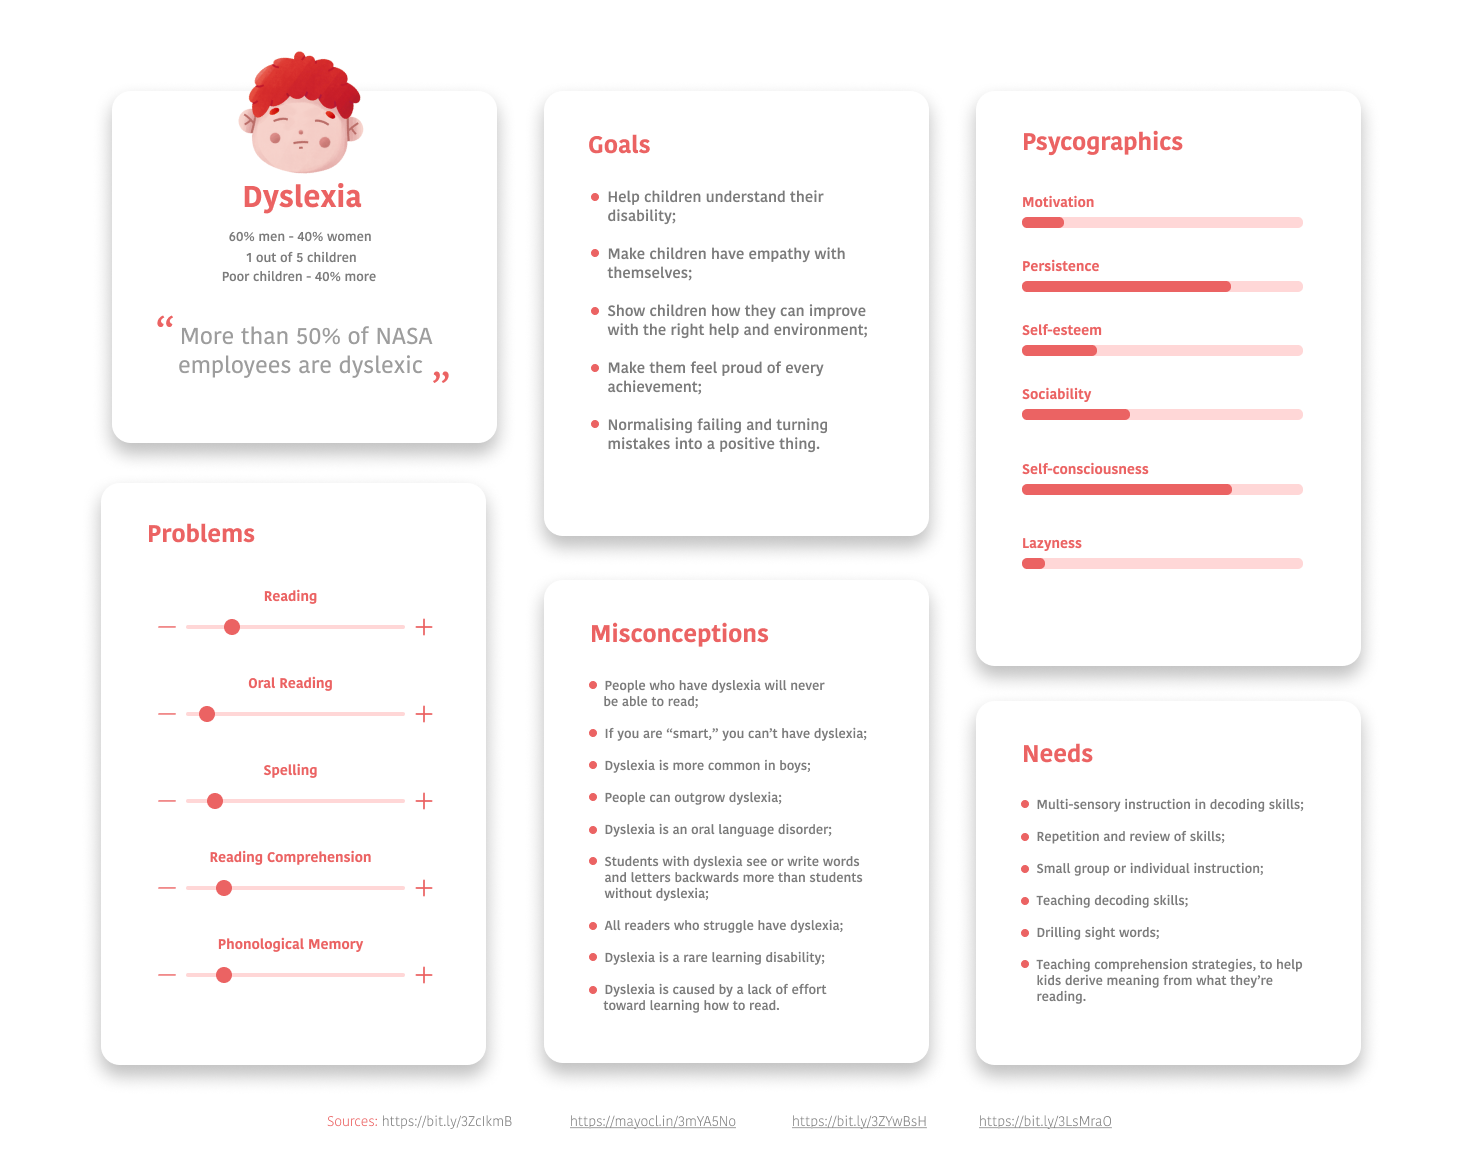
\includegraphics[width=0.8\linewidth]{Chapters/figma/Dislexia.png}
    \caption{Dyslexia User Profile}
    \label{fig:dyslexiaUserProfile}
\end{figure}

\paragraph{\textbf{Goals}}
\begin{itemize}
    \item \textbf{Help children understand their disability}: The mini-games aim to provide children with a clear understanding of dyslexia, its effects on reading, and how it does not define their intelligence or potential.
    \item \textbf{Foster empathy and self-acceptance}: By creating an environment that encourages self-compassion and understanding, the mini-games aim to instill a sense of empathy within children towards themselves and others facing similar challenges.
    \item \textbf{Promote improvement through appropriate support}: The mini-games strive to demonstrate how with the right help and a supportive environment, children with dyslexia can make significant improvements in their reading abilities.
    \item \textbf{Cultivate a sense of achievement}: Recognizing and celebrating every milestone and achievement, no matter how small, is a key objective of the mini-games.
    \item \textbf{Normalize failure and embrace mistakes}: The mini-games aim to shift the perception of failure by illustrating that mistakes are an inherent part of the learning process and can lead to positive growth.
\end{itemize}

\paragraph{\textbf{Psycographics}}
\begin{itemize}
    \item \textbf{Low self-esteem}: Dyslexia can negatively impact self-esteem due to difficulties experienced in reading and academic settings. \cite{dyslexiaUnderstanding}
    \item \textbf{High persistence}: Children with dyslexia often exhibit determination and persistence in overcoming challenges related to reading. \cite{dyslexiaStatistics}
    \item \textbf{Medium-low sociability}: Children with dyslexia may exhibit varying levels of sociability, often preferring smaller social groups or activities that do not heavily rely on reading. \cite{dyslexiaClinic}
    \item \textbf{High self-consciousness}: Dyslexia can make children self-conscious about their reading abilities, leading to heightened self-awareness in educational settings.
    \item \textbf{Low laziness}: Despite the challenges they face, children with dyslexia typically demonstrate a strong work ethic and a drive to overcome difficulties. \cite{dyslexiaStatistics}
\end{itemize}

\paragraph{\textbf{Problems}}
\begin{itemize}
    \item \textbf{Reading}: Difficulties in accurately and fluently recognizing and decoding words. \cite{dyslexiaCharAndSigns}
    \item \textbf{Reading Aloud}: Challenges in pronouncing words correctly and maintaining fluency while reading aloud. \cite{dyslexiaCharAndSigns}
    \item \textbf{Spelling}: Struggles with accurate spelling due to difficulties in connecting sounds to letters and understanding spelling patterns. \cite{dyslexiaCharAndSigns}
    \item \textbf{Reading Comprehension}: Difficulties in understanding and deriving meaning from written text, impacting overall comprehension skills.\cite{dyslexiaCharAndSigns}
    \item \textbf{Phonological Memory}: Challenges in remembering and manipulating speech sounds, affecting phonemic awareness and decoding skills. \cite{dyslexiaCharAndSigns}
\end{itemize}

\paragraph{\textbf{Facts}}
\begin{itemize}
    \item Dyslexia does not prevent individuals from learning how to read. \cite{dyslexiaCharAndSigns}
    \item Intelligence is not a determining factor in the presence of dyslexia. \cite{dyslexiaStatistics}
    \item Dyslexia affects both boys and girls. \cite{dyslexiaCharAndSigns}
    \item Dyslexia is a lifelong learning disability, but individuals can make significant progress with appropriate interventions and support. \cite{dyslexiaCharAndSigns}
    \item Dyslexia primarily affects reading, not oral language skills. \cite{dyslexiaCharAndSigns}
    \item Reversing letters or words is not exclusive to dyslexia. \cite{dyslexiaCharAndSigns}
    \item Dyslexia is a relatively common learning disability.
    \item Dyslexia is not caused by a lack of effort or motivation to learn how to read.
\end{itemize}

\paragraph{\textbf{Needs}}
\begin{itemize}
    \item \textbf{Multi-sensory instruction in decoding skills}: Children with dyslexia benefit from instructional approaches that engage multiple senses simultaneously. This approach typically involves integrating visual, auditory, and kinesthetic modalities to reinforce letter-sound relationships and improve reading accuracy. For example, a mini-game could present letters or words visually while simultaneously providing auditory feedback or encouraging physical manipulation of letter tiles. \cite{dyslexiaUnderstanding}
    \item \textbf{Repetition and review of skills}: Dyslexic learners require ample opportunities for practice and reinforcement of decoding skills. Repetition helps solidify their understanding of letter-sound associations, spelling patterns, and reading strategies. Mini-games can incorporate repeated exposure to target skills through varied and engaging activities, allowing children to reinforce their learning in an interactive and enjoyable manner. \cite{dyslexiaUnderstanding}
    \item \textbf{Small group or individual instruction}: Dyslexia-specific instruction often benefits from personalized attention in small group settings or one-on-one instruction. Mini-games can be designed to accommodate different group sizes, allowing for targeted interventions and tailored support. Providing individualized feedback and adaptive features within the games can further enhance the effectiveness of small group or individual instruction. \cite{dyslexiaUnderstanding}
    \item \textbf{Teaching decoding skills}: Dyslexic children often struggle with decoding, the process of translating written words into spoken language. Mini-games can focus on teaching and reinforcing decoding skills by incorporating activities that require the identification and blending of letter sounds, syllables, or whole words. Interactive feedback and scaffolding mechanisms can guide children through the decoding process, promoting accuracy and fluency. \cite{dyslexiaUnderstanding}
    \item \textbf{Drilling sight words}: Sight words, also known as high-frequency words, are common words that dyslexic learners encounter frequently but do not follow regular phonetic patterns. Mini-games can include drills and practice exercises that specifically target sight words. By presenting these words repeatedly in engaging formats, such as word recognition games or word-building puzzles, dyslexic learners can improve their automatic recognition and reading fluency. \cite{dyslexiaUnderstanding}
    \item \textbf{Teaching comprehension strategies to help derive meaning from text}: Reading comprehension is a significant challenge for individuals with dyslexia. Mini-games can incorporate activities that teach and reinforce comprehension strategies, such as identifying main ideas, making inferences, summarizing information, and visualizing text. By practicing these strategies within interactive game contexts, children with dyslexia can develop stronger comprehension skills and derive meaning from what they read. \cite{dyslexiaUnderstanding}
\end{itemize}

% https://www.fcps.edu/academics/academic-overview/special-education-instruction/high-incidence-disabilities-team-k-12-2
% https://www.mayoclinic.org/diseases-conditions/dyslexia/symptoms-causes/syc-20353552
% https://childmind.org/article/understanding-dyslexia/
% https://www.crossrivertherapy.com/research/dyslexia-statistics
% Add image

% \begin{itemize}
%     \item \textbf{Goals}
%     \begin{itemize}
%         \item \textbf{Help children understand their disability}: The mini-games aim to provide children with a clear understanding of dyslexia, its effects on reading, and how it does not define their intelligence or potential.
%         \item \textbf{Foster empathy and self-acceptance}: By creating an environment that encourages self-compassion and understanding, the mini-games aim to instill a sense of empathy within children towards themselves and others facing similar challenges.
%         \item \textbf{Promote improvement through appropriate support}: The mini-games strive to demonstrate how with the right help and a supportive environment, children with dyslexia can make significant improvements in their reading abilities.
%         \item \textbf{Cultivate a sense of achievement}: Recognizing and celebrating every milestone and achievement, no matter how small, is a key objective of the mini-games.
%         \item \textbf{Normalize failure and embrace mistakes}: The mini-games aim to shift the perception of failure by illustrating that mistakes are an inherent part of the learning process and can lead to positive growth.
%     \end{itemize}
%     \item \textbf{Psycographics}
%     \begin{itemize}
%         \item \textbf{High persistence}: Children with dyslexia often exhibit determination and persistence in overcoming challenges related to reading.
%         \item \textbf{Low self-esteem}: Dyslexia can negatively impact self-esteem due to difficulties experienced in reading and academic settings.
%         \item \textbf{Medium-low sociability}: Children with dyslexia may exhibit varying levels of sociability, often preferring smaller social groups or activities that do not heavily rely on reading.
%         \item \textbf{High self-consciousness}: Dyslexia can make children self-conscious about their reading abilities, leading to heightened self-awareness in educational settings.
%         \item \textbf{Low laziness}: Despite the challenges they face, children with dyslexia typically demon   strate a strong work ethic and a drive to overcome difficulties.
%     \end{itemize}
%     \item \textbf{Problems}
%     \begin{itemize}
%         \item \textbf{Reading}: Difficulties in accurately and fluently recognizing and decoding words.
%         \item \textbf{Reading Aloud}: Challenges in pronouncing words correctly and maintaining fluency while reading aloud.
%         \item \textbf{Spelling}: Struggles with accurate spelling due to difficulties in connecting sounds to letters and understanding spelling patterns.
%         \item \textbf{Reading Comprehension}: Difficulties in understanding and deriving meaning from written text, impacting overall comprehension skills.
%         \item \textbf{Phonological Memory}: Challenges in remembering and manipulating speech sounds, affecting phonemic awareness and decoding skills.
%     \end{itemize}
%     \item \textbf{Misconceptions}
%     \begin{itemize}
%         \item Dyslexia does not prevent individuals from learning how to read.
%         \item Intelligence is not a determining factor in the presence of dyslexia.
%         \item Dyslexia affects both boys and girls.
%         \item Dyslexia is a lifelong learning disability, but individuals can make significant progress with appropriate interventions and support.
%         \item Dyslexia primarily affects reading, not oral language skills.
%         \item Reversing letters or words is not exclusive to dyslexia.
%         \item Dyslexia is a relatively common learning disability.
%         \item Dyslexia is not caused by a lack of effort or motivation to learn how to read.
%     \end{itemize}
%     \item \textbf{Needs}
%     \begin{itemize}
%         \item \textbf{Multi-sensory instruction in decoding skills}: Children with dyslexia benefit from instructional approaches that engage multiple senses simultaneously. This approach typically involves integrating visual, auditory, and kinesthetic modalities to reinforce letter-sound relationships and improve reading accuracy. For example, a mini-game could present letters or words visually while simultaneously providing auditory feedback or encouraging physical manipulation of letter tiles.
%         \item \textbf{Repetition and review of skills}: Dyslexic learners require ample opportunities for practice and reinforcement of decoding skills. Repetition helps solidify their understanding of letter-sound associations, spelling patterns, and reading strategies. Mini-games can incorporate repeated exposure to target skills through varied and engaging activities, allowing children to reinforce their learning in an interactive and enjoyable manner.
%         \item \textbf{Small group or individual instruction}: Dyslexia-specific instruction often benefits from personalized attention in small group settings or one-on-one instruction. Mini-games can be designed to accommodate different group sizes, allowing for targeted interventions and tailored support. Providing individualized feedback and adaptive features within the games can further enhance the effectiveness of small group or individual instruction.
%         \item \textbf{Teaching decoding skills}: Dyslexic children often struggle with decoding, the process of translating written words into spoken language. Mini-games can focus on teaching and reinforcing decoding skills by incorporating activities that require the identification and blending of letter sounds, syllables, or whole words. Interactive feedback and scaffolding mechanisms can guide children through the decoding process, promoting accuracy and fluency.
%         \item \textbf{Drilling sight words}: Sight words, also known as high-frequency words, are common words that dyslexic learners encounter frequently but do not follow regular phonetic patterns. Mini-games can include drills and practice exercises that specifically target sight words. By presenting these words repeatedly in engaging formats, such as word recognition games or word-building puzzles, dyslexic learners can improve their automatic recognition and reading fluency.
%         \item \textbf{Teaching comprehension strategies to help derive meaning from text}: Reading comprehension is a significant challenge for individuals with dyslexia. Mini-games can incorporate activities that teach and reinforce comprehension strategies, such as identifying main ideas, making inferences, summarizing information, and visualizing text. By practicing these strategies within interactive game contexts, children with dyslexia can develop stronger comprehension skills and derive meaning from what they read.
%     \end{itemize}
% \end{itemize}
